\documentclass[tikz,border=10pt]{standalone}
\usepackage{tkz-euclide} % 引入几何增强包

\begin{document}
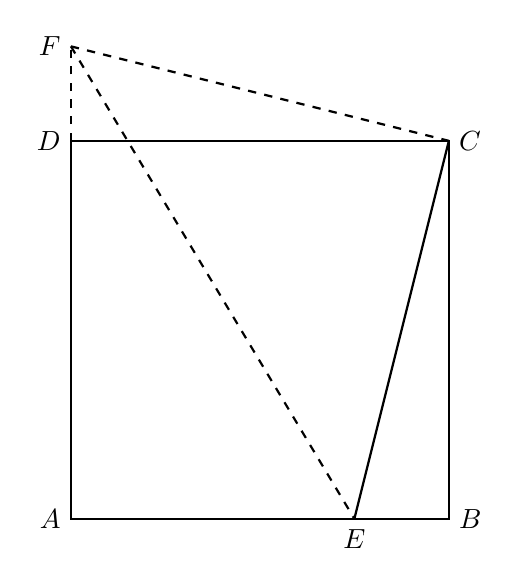
\begin{tikzpicture}[scale=1.2, thick, >=stealth]
    % 1. 定义核心点坐标 (以 A 为原点)
    \coordinate (A) at (0,0);
    \coordinate (B) at (4,0);
    \coordinate (C) at (4,4);
    \coordinate (D) at (0,4);
    
    % 定义 E 点 (在 AB 上，假设 AE = 3)
    \coordinate (E) at (3,0);
    
    % 定义 F 点 (在 AD 的延长线上，假设 DF = 1)
    \coordinate (F) at (0,5);

    % 2. 绘制实线部分 (四边形和内部连线)
    \draw (A) -- (B) -- (C) -- (D) -- cycle;
    \draw (C) -- (E);

    % 3. 绘制虚线部分 (辅助线)
    \draw[dashed] (D) -- (F);  % AD 的延长线部分
    \draw[dashed] (F) -- (C);  % 连线 FC
    \draw[dashed] (F) -- (E);  % 连线 FE

    % 4. 标注文本标签
    % anchor 用于微调文字位置，避免覆盖线条
    \node[left] at (A) {$A$};
    \node[right] at (B) {$B$};
    \node[right] at (C) {$C$};
    \node[left] at (D) {$D$};
    \node[below] at (E) {$E$};
    \node[left] at (F) {$F$};

    % 5. 可选：绘制直角标记 (根据题目需求决定是否开启)
    % \draw (0,0.2) -- (0.2,0.2) -- (0.2,0); % A点直角
\end{tikzpicture}
\end{document}